\documentclass[notitlepage]{article}

\usepackage{color, listings, bm, amsmath, blkarray, gensymb}
% \usepackage[percent]{overpic}
\usepackage{tikz, lineno, natbib, url}
\linenumbers
% \usepackage{graphicx}
% \usepackage{epsfig}
% \usepackage{subfig}
% \captionsetup{belowskip=12pt}
% \hfuzz=5.002pt  %suppress overfull warnings

\author{Michael Vlah}
\title{Determining multi-scale controls on river temperature: a time series approach}

\begin{document}
\pagenumbering{gobble}
% todo:
% include snowmelt in model run. see if it's worth including with precip and temp as a climate predictor
% introduce terminology:
% responses = water temp, Q
% climatic predictors = air temp, precip, drought
% landscape predictors = many
%include hydrograph figures from kathy liederman and julian olden to show
    %rain dom, rain and snow, snow dom
%include the over-time plots in the supplemental information
%in regression figure, line up left side of legend box with plot above
    %make gray horiz line go only to topright corner of box
    %make axis lines and plot borders cleaner (right now axis segments are darker)
    %instead of elevation on x, use ice and color by elev (orange to blue) X no story
    %for loadings, color by ice and make it darkgreen , midgreen, white X not without the above
    % add % ice as one of the hidden trends
%discharge regression combo plot is scrapped. no relationship with snowmelt?
%discharge only really relevant in the Q v temp plot.
%increase unit text size in fig 2
%change area over 1000m to % area over 1000m and replot
%change "dominated" to "dominant"
%change "fall" to "autumn"
%dont size points in figure 2. include size in legend in fig 3
%adjust letter position in corners of fig 2 (anchoring)
%see if its possible to directly compare Z and D
%include the average effect size of tair on twater in 3a
% can i say how much elevation would inflence temperature independent of snowmelt?
%examine change over time in just the elwha
%%%%why am i removing additional seasonal variation (fixed factor)???
%probably get snowmelt out of the picture? it may be misleading and a source of criticism
%explain why some SD rivers might have a larger effect than RD (related to slope, groundwater?)
%get snowmelt out of there. it's a watershed trait. not a regional one
%add discharge locations to the map?
%probably should include a table of data sources and station ids

\maketitle
\vspace{10pc}
\noindent
\textbf{Summary:}

\noindent
5 data sources; watershed delineation; 2 DFAs: m=1:15, 7 covariate combinations, 4 err. struc., 2 seasonality models; TMB; parallel computing; Bayesian change/time
\clearpage
\pagenumbering{arabic}

\section*{Abstract}
Temperature is among the most important determinants of riverine biodiversity and health. It is therefore a primary freshwater management concern, particularly where cold-water fish are of high ecological, recreational, and commercial value. However, river temperature in the Puget Sound watershed of the Northwestern U.S.A. is affected by a great diversity of drivers at multiple spatial and temporal scales, and little is known of their interactions. We used dynamic factor analysis, a multivariate time-series technique, to examine relationships among these drivers, synthesizing long-term climate and fine-scale landcover data. We found that primarily rain-fed rivers experience large seasonal temperature fluctuations, which closely track atmospheric temperature, while snow-fed rivers tend to be weakly, and in some cases inversely, coupled with such fluctuations. Among watersheds, groundwater influx, land slope, and discharge further augment or dampen these relationships. Our results suggest the temperature of high-elevation rivers, absent the influence of ice, should be highly variable, and that glacially fed streams stand to see the largest changes in temperature regime under proposed climate scenarios.
\clearpage

\section*{Introduction}

The ecological condition of a stream or river, the life it supports, and the goods and services it provides, are influenced by the timing and magnitude of seasonal changes in water temperature. Temperature is a chief consideration in the management of fisheries, as it affects species distribution \citep{Boisneau2008}, growth and reproduction \citep{mccullough1999review}, and migration timing \citep{boscarino2007effects}. In particular, In the Puget Sound watershed of the American Pacific Northwest, several salmonid species spawn, migrate, and emerge only within the bounds of a few degrees Celsius, and thrive under even greater temperature constraints \citep{carter2005effects}. As a result, the success of commercial and recreational fisheries that depend on the region's riverine habitat rests on many precarious factors.

River networks, being fractal in structure, are naturally governed by environmental processes at multiple scales. Seasonal variation in water temperature in rivers of the Pacific Northwest is a function of the surrounding air, as well as precipitation and snowmelt \citep{eldridge1967water}. These drivers may in turn be mediated or supplemented by several aspects of watershed morphology at smaller scales, including slope, elevation, and geology \citep{poole2001ecological,lisi2013association}. Taken together, this hierarchical system complicates fishery management, as the temperature regime of one river may be the direct product of climate, while that of another may depend more on within-watershed conditions.

Adding to this picture, flow regimes across rivers of the Puget Sound watershed vary with latitude and elevation \citep{reidy2012hydrogeomorphic,mauger2015CIG}, and can be classified broadly into three categories by flow source and hydrograph shape. Rain-dominated (RD) rivers receive little or no input from snowmelt, and thus peak in discharge during the rainy season, usually between October and February. Snow-dominated (SD) rivers instead see peak flow during spring snowmelt, often in April, May, or June. Between these extremes lies a third class of rain-and-snow-driven (RS) rivers, which have appreciable peaks at both times.

Effective management plans must therefore integrate a diversity of factors across space and time in order to determine which rivers and watersheds are likely to see consequential changes under projected climate and land use scenarios for the Pacific Northwest \citep{mote2010future,radeloff2012economic}. However, the understanding required to do so is limited by knowledge of relationships among temperature drivers at scale.

% The physical properties of water also change with temperature, which measurably affects the efficacy of electrical power generation (Foerster & Lillestam 2010), and drinking water production (Ramaker et al. 2005).
% Physically, temperature determines vapor pressure, surface tension, density (Stevens et al. 1975), gas solubility, reaction rates (Brezonik 1972) and more.

We sought to identify streams in the Puget Sound region whose temperatures fluctuate closely with regional trends in air temperature, precipitation, and snowmelt, and those that depart from regional patterns. Our second aim was to identify watershed features that correlate with such departures, and thus provide a nuanced basis for predicting impacts of water temperature on aquatic biodiversity and fishery health. We hypothesized that water temperature would track air temperature most closely in RD rivers \citep{ward1985thermal,garner2014river}. We expected deviations from this relationship to correlate best with cold-water influx from snow and ice melt \citep{lisi2015watershed} and with factors affecting heat capacity of water, including discharge (volume over time) and watershed slope (which relates to turbulence, surface area, and mixing; \citealt{van2013global}).

%carter 2005 http://www.swrcb.ca.gov/northcoast/water_issues/programs/tmdls/shasta_river/060707/28appendixaetheeffectsoftemperatureonsteelheadtroutcohosalmonandchinooksalmonbiologyandfunction.pdf:
    %usepa 1999

\section*{Methods}

% \subsection*{Study region and climate data}

% Monthly time series of mean and max air temperature (\degree C), total precipitation (cm), snowmelt (cm), and hydrological drought (Palmer Hydrological Drought Index) were acquired for the time-span of 1978 to 2015.

% https://wa.water.usgs.gov/data/realtime/adr/interactive/ #discharge daily
% https://waecy.maps.arcgis.com/apps/Viewer/index.html?appid=832e254169e640fba6e117780e137e7b #Q 15min
% http://www.horizon-systems.com/NHDPlus/NHDPlusV2_17.php #nhdplus
% ftp://newftp.epa.gov/EPADataCommons/ORD/NHDPlusLandscapeAttributes/StreamCat/HydroRegions/ #streamca
% ncdc.noaa.gov/cag/time-series/us #climate data
% https://www.nrcs.usda.gov/wps/portal/nrcs/detail/or/snow/?cid=nrcs142p2_046350 #snow
% https://arxiv.org/pdf/1509.00660.pdf #TMB
% Harvey, A. C. 1989. Forecasting, structural time series models and the Kalman flter. Cambridge University Press, Cambridge, UK.
%CIG puget sound state of knowledge http://cses.washington.edu/picea/mauger/ps-sok/ps-sok_sec03_watercycle_2015.pdf

\subsection*{Water and climate data}

We investigated climate and landscape controls on water temperature and discharge, as separate response variables, from 1978 to 2015. Monthly time series of water temperature were obtained for 24 river sites via the Washington Department of Ecology's River and Stream Water Quality Monitoring program \citep{DoEwaterData}. These sites represent 19 nonnested watersheds across 9 counties, and range from 4 to 775 m in elevation. For at least one site at each river, monthly discharge time series were also available, either from the same location as one of the temperature monitoring sites, or from within 30 km on the same major reach. Discharge data were aggregated by monthly mean from the USGS National Water Information System database \citep{USGSdischarge}.

\begin{center}
\resizebox{\textwidth}{!}{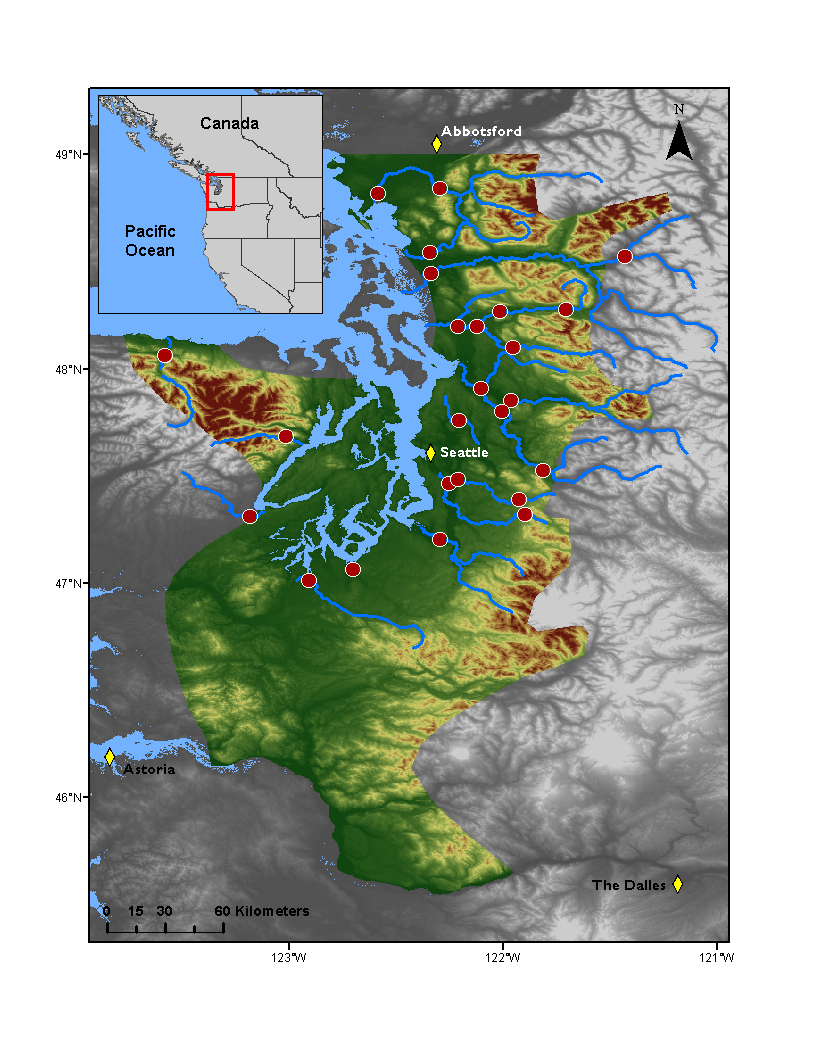
\includegraphics{figures/map/map.png}}
\textbf{Figure 1} Site locations (red points) in relation to combined Washington State Climate Divisions 3 and 4 (colored topography), the region across which climate data were aggregated.
\end{center}

Potential climatic predictors of water temperature and discharge included mean and max air temperature (\degree C), total precipitation (cm), snowmelt (cm), and hydrological drought (Palmer Hydrological Drought Index), averaged by month across the response variable time series. All but snowmelt were available through the U.S. Climate Divisional Dataset, developed by the National Centers for Environmental Information (NCEI; \citealt{climateData}). We acquired climatic predictor data grouped by Washington State climate division, and all but two of our sites fell within divisions 3 (Puget Sound Lowland) and 4 (East Olympic/Cascade Foothills; see Fig. 1). We therefore aggregated these data by monthly mean across the two regions (after verifying their post-standardization similarity), resulting in a single dataset of four climatic predictor variables. A snowmelt time series was then added to this dataset, using monthly mean records from six SNOTEL sites (Bumping Ridge, Elbow Lake, Mount Crag, Park Creek Ridge, Stevens Pass, White Pass) listed by the USDA's Natural Resources Conservation Service; \citealt{snowData}. We calculated monthly snowmelt for each site as the absolute value of negative differences in cumulative snow water equivalent from each month to the next. The snowmelt time series was assigned zeros for any positive differences (accumulations).

%More information on all datasets can be found in \colorbox{red}{\lstinline{Appendix A}}.

\subsection*{Time series analysis}
Response time series were modeled using dynamic factor analysis (DFA; \citealt{zuur2003estimating}), a multivariate technique that can be thought of as an analog to principal component analysis in the time domain. In DFA, response time series are fit with a linear combination of shared, random-walk trends (usually many fewer than the total number of response series), predictors (which can have unique effects on each response series), and random error. We chose DFA over a traditional multivariate state space approach for two reasons. First, it provides advantages in computational efficiency, as a small number of shared trends often adequately capture variation across dozens of responses, and at much lower parameter cost \citep{zuur2003dynamic}. Second, in terms of identifying what drives the shared trends, having fewer of them allows for greater inferential parsimony. Being a multivariate technique, DFA also provides an advantage over univariate alternatives in that covariance structure among responses can be specified and compared. All models were fit using maximum likelihood estimation by automatic differentiation, with Template Model Builder software \citep{kristensen2015tmb}, which we called using package TMB in R \citep{Rmanual,tmbPackage}.

DFA takes the following form:

\begin{equation}
    \textbf{x}_t = \textbf{x}_{t-1} + \textbf{w}_t\textrm{, where } \textbf{w}_t \sim \textrm{MVN}(0,\textbf{Q})
\end{equation}
\begin{equation}
    \textbf{y}_t = \textbf{Zx}_t + \textbf{Dd}_t + \textbf{v}_t\textrm{, where } \textbf{v}_t \sim \textrm{MVN}(0,\textbf{R})
\end{equation}
\begin{equation}
    \textbf{x}_0 \sim \textrm{MVN}(0,\bm{\Lambda})
\end{equation}

At time step {\it t}, the $m \times 1$ vector of shared trends (\textbf{x}) is a function of \textbf{x} in the previous step, plus normal error (\textbf{w}; $m\times 1$; Eq. 1). This is the definition of a random walk. The $n\times 1$ response vector (\textbf{y}) at time {\it t} is a function of the shared trends and their factor loadings (\textbf{Z}; $n\times m$), covariates (\textbf{d}; $q\times 1$) and their river-specific effects (\textbf{D}; $n\times q$), and a second normal error term (\textbf{v}; $n\times 1$; Eq. 2). \textbf{R} and \textbf{Q} are variance-covariance matrices of order m, and \textbf{Q} is set to identity for model identifiability \citep{harvey1990forecasting}. The initial state of the shared trend vector ($\bm{x}_0$) is multivariate-normally distributed with a mean of zero and a diagonal variance-covariance matrix with large variance (e.g. 5; Eq. 3). Response and predictor data were standardized to facilitate comparison of effect sizes and avoid error inflation.

% Response data were centered on 0, but not scaled, to avoid error inflation \colorbox{red}{\lstinline{details and citation}}.

Because we were interested in isolating the effects of climatic predictors on river temperature and discharge, we used fixed factors to absorb recurring seasonal variation not related to the predictors, with one factor level for each month. These factors were incorporated into the covariate matrix (\textbf{d}). Thus, the coefficient in \textbf{D} relating, say, air temperature (predictor) and water temperature (response), represents the effect size of the former on the latter. In other words, it is the change in water temperature accompanying a unit change in air temperature across the whole time series. We call this relationship "coupling." We were also interested in coupling by month for specific predictors, which required that the focal predictor in a particular model be arranged seasonally. Concretely,

$$
\textbf{d} = \begin{blockarray}{cccccc}
& \textrm{Jan}_{1978} & \textrm{Feb}_{1978} & \textrm{Mar}_{1978} & \cdots & \textrm{Dec}_{2015} \\
\begin{block}{c(ccccc)}
    1 & 1 & 0 & 0 & \cdots & 0 \\
    2 & 0 & 1 & 0 & \cdots & 0 \\
    3 & 0 & 0 & 1 & \cdots & 0 \\
      & \vdots & \vdots & \vdots & \ddots & \vdots \\
    12 & 0 & 0 & 0 & \cdots & 1 \\
    13 & \theta_{precip}^{(1)} & \theta_{precip}^{(2)} & \theta_{precip}^{(3)} & \cdots & \theta_{precip}^{(T)} \\
    14 & \theta_{air}^{(1)} & 0 & 0 & \cdots & 0 \\
    15 & 0 & \theta_{air}^{(2)} & 0 & \cdots & 0 \\
    16 & 0 & 0 & \theta_{air}^{(3)} & \cdots & 0 \\
      & \vdots & \vdots & \vdots & \ddots & \vdots \\
    25 & 0 & 0 & 0 & \cdots & \theta_{air}^{(T)} \\
\end{block}
\end{blockarray}
$$

is the covariate matrix structure necessary to account for exogenous seasonal variation (rows 1-12), and overall effect of precipitation (row 13), while also yielding the by-month effect of air temperature (rows 13-24) on the response (\textbf{y}).

Additional, non seasonal variation due to exogenous effects loads onto the shared trends, and a portion of remaining variation is absorbed by error matrix \textbf{v}. We fit models using four unique error structures (\textbf{R}), to allow for different suites of unknown drivers affecting rivers. We included shared variance and zero covariance, individual variance and zero covariance, shared variance and shared covariance, and unconstrained error. Details on these structures and their implications can be found in \citep{holmes2012marss}. The best models for water temperature and discharge were determined with AIC.

\subsection*{Landscape predictors and post-hoc regression}

For post-hoc analyses, monitoring sites were separated into three classes based on relative areal coverage of perennial ice and/snow (hereinafter ``\% glaciation'') and mean elevation across their watersheds. The three classes are loosely based on the classification scheme and language of the Climate Impacts Group at the University of Washington \citep{mauger2015CIG}, and are here delineated according to Table 1.

% \begin{table}
\begin{center}
\textbf{Table 1} Watershed classification scheme
\end{center}
\begin{center}
\begin{tabular}{ |c|c|c|c| }
 \hline
 Classification & Abb. & Glaciation (\%) & Mean elev. (m) \\
 \hline
 Rain-dominated & RD & $< 0.7$ & $< 600$ \\
 Rain-and-snow & RS & $< 0.7$ & $\geq 600$ \\
 Snow-dominated & SD & $\geq 0.7$ & - \\
 \hline
\end{tabular}
\end{center}
% \end{table}

After model selection, climatic predictor effect sizes for each river were back-transformed to their original scales and regressed against landscape predictors in order to identify possible watershed-scale controls on coupling. To achieve this, we amassed an additional dataset of landscape features. These were collected individually for each of the watersheds corresponding to our 24 river sites, using the EPA's StreamCat (stream-catchment) data library \citep{hill2016stream} and the National Hydrography Dataset (NHDPlusV2; \citealt{mckay2012nhdplus}). Each site was mapped to an individual river reach, defined as a segment bounded on each end by a stream or river source, confluence, or mouth. The region contributing flow to this reach (its watershed) was then fetched, along with selected areal data, from the NHDPlusV2 database. Landscape attributes used as predictors were aggregated by watershed mean where applicable, and include elevation (m), total area (km\textsuperscript{2}), base flow index, soil permeability (cm hr\textsuperscript{-1}), water table depth (cm), bedrock depth (cm), Base Flow Index (BFI; \%), runoff (mm mo\textsuperscript{-1}), percent perennial ice and snow coverage (National Land Cover Database [NLDC] 2006 and 2011 average), riparian population density (people km\textsuperscript{-2} within 100m of streams; 2010 census), riparian road density (km km\textsuperscript{-2}; 2010 census), and percent riparian urban land (NLCD 2011). Monitoring site elevation (m) and presence of upstream dams (as full/partial/no damming of upstream mainstem and major tributaries) were also included. Finally, we calculated \% area over 1000 m (km\textsuperscript{2}), mean slope (percent rise), and mean aspect (degree) by delineating watersheds from a digital elevation model in ArcMap version 10.4 \citep{arcviewenvironmental}.

\section*{Results}

Mean monthly temperature trends for the three river classes, aggregated across all 38 years of data, deviated by a minimum of 1.0\degree C in December, and a maximum of 3.9\degree C in July (Fig. 2). SD rivers remained approximately two degrees colder than their RS counterparts through mid-late summer, and 3-4 degrees colder than RD throughout spring and summer. RD rivers were consistently warmest throughout the year. In January, RS reached a minimum of 4.4\degree C, and did not significantly differ from SD (Student's t: $p<0.01, F=11.9$). RD, meanwhile, only attained a minimum of 5.6\degree C. RS reached a peak summer temperature of 16.9\degree C in July, while RS and SD followed in August with peak temperatures of 15.5 and 13.5\degree C, respectively.

Meanwhile, the amplitude of T\textsubscript{air} oscillation exceeded that of any river class, dipping below T\textsubscript{water} in autumn to a minimum of 3.2\degree C in December, and rising above RS and SD in March to an August maximum of 17.4\degree C. T\textsubscript{air} did not overtake RD T\textsubscript{water} until August, by which time the latter had begun to decline.

% \begin{figure}[h!]
\begin{center}
% 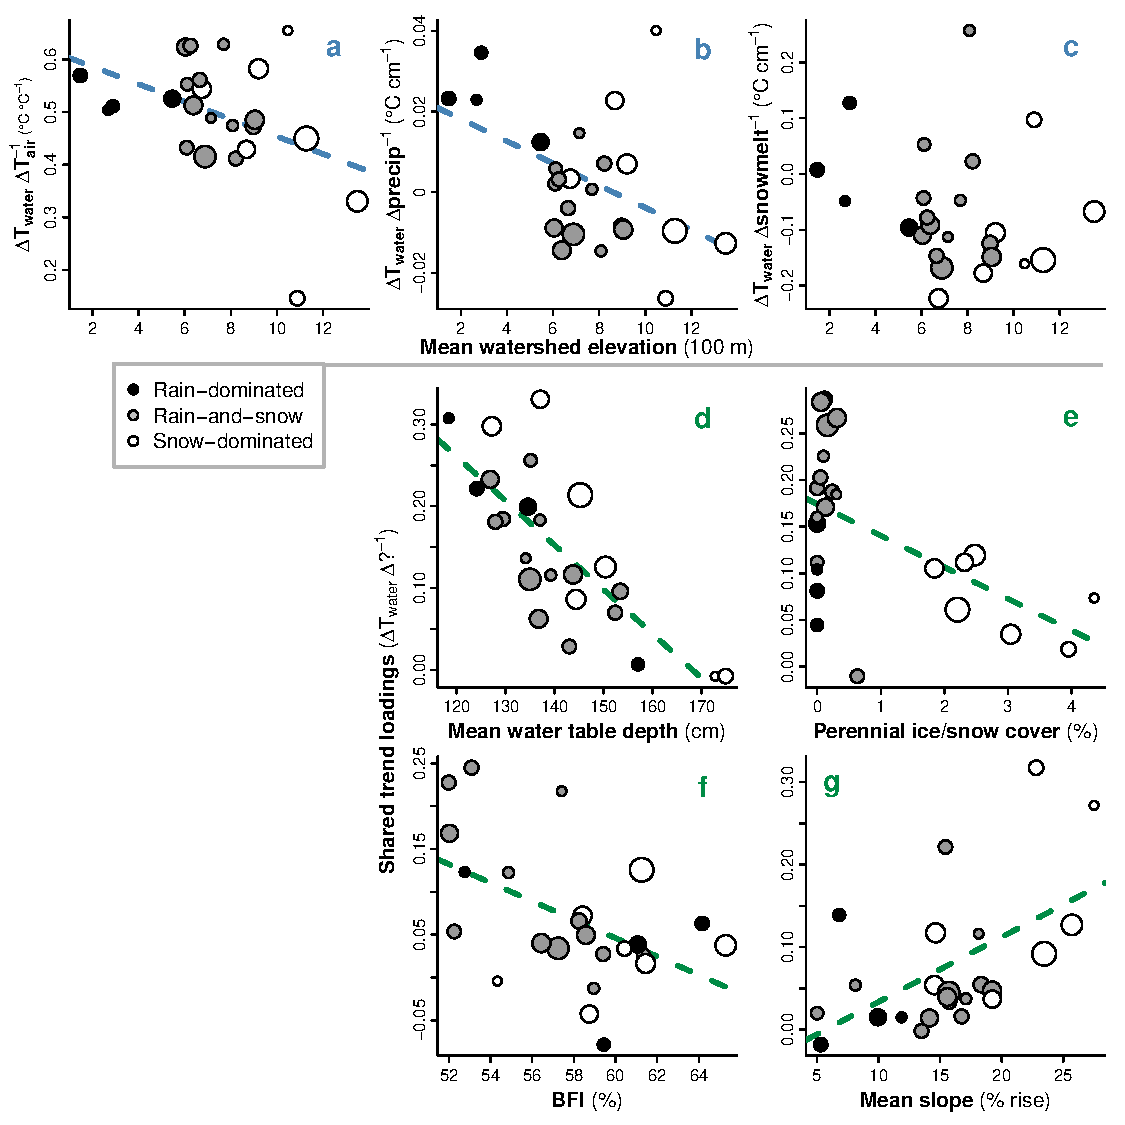
\includegraphics[width=\textwidth]{figures/16_temp_all_reg.pdf}
\resizebox{\textwidth}{!}{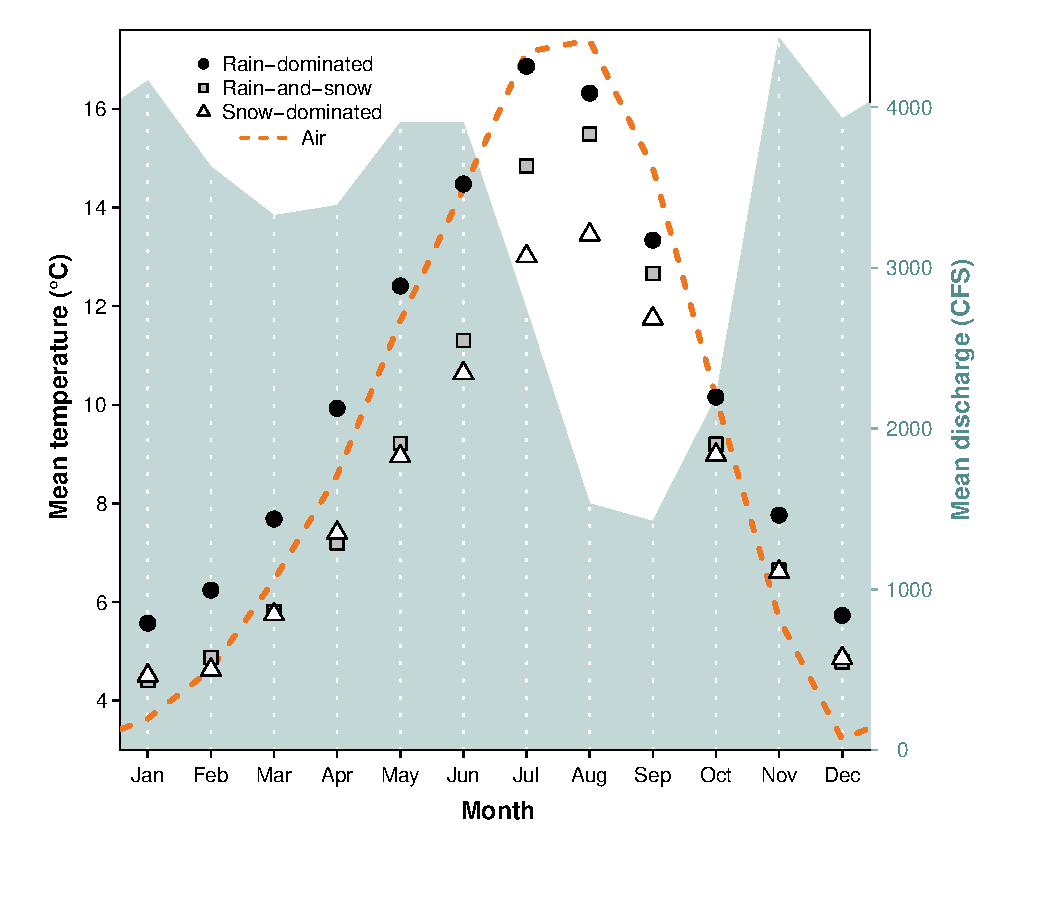
\includegraphics{figures/12_air_water_discharge.pdf}}
% \caption{Epipolar Geometry}
% \label{fig:air_water_disch}
\end{center}
% \end{figure}

\textbf{Figure 2} Monthly mean T\textsubscript{water} by river class, and T\textsubscript{air} and Q across classes, from 1978 to 2015. All depicted series represent discrete data. \setlength{\parskip}{6pt}\\[\baselineskip]
% see appendix for standard deviations?

The combined hydrograph of all rivers reveals two primary peaks, one beginning in late spring and the other extending from late fall to early winter, with a prominent trough in late summer. Spring peak discharge coincides noticeably with a separation in water temperature between SD and RS, while the summer trough coincides with separation of RD and T\textsubscript{air}. November marks both the autumn peak in discharge and the point at which T\textsubscript{air} falls below T\textsubscript{water}.

\sloppy
DFA results, aggregated across months and years for each site, revealed a trend toward reduced $T_{air}\rightarrow T_{water}$ coupling with greater watershed elevation ($p=0.04, R^2=0.18$; Fig. 3a). On average, a 1\degree C change in T\textsubscript{air} corresponded to a $0.53\pm 0.03$\degree C change in T\textsubscript{water} at RD, a $0.51\pm 0.08$\degree C change at RS, and a $0.45\pm 0.17$\degree C change at SD sites. A similar trend was observed with respect to $Precip\rightarrow T_{water}$ coupling ($p=0.03, R^2=0.21$; Fig. 3b), where a monthly change in total precipitation of 1 cm corresponded to a $0.02\pm 0.009$\degree C change in T\textsubscript{water} for RD, $-0.003\pm 0.009$\degree C for RS, and $0.004\pm 0.02$\degree C for SD. There was no evidence of coupling between snowmelt and T\textsubscript{water} (Fig. 3c), but this predictor was included in the most parsimonious DFA model selected via AIC and R\textsuperscript{2} (See Appendix A.). It is of note that the strongest examples of $T_{air}\rightarrow T_{water}$ and $Precip\rightarrow T_{water}$ coupling were observed in the Duckabush River, while the weakest examples are from the Elwha River. Both rivers drain glaciers of the Olympic Mountain Range, and both are SD, though the Elwha's watershed is larger.

\begin{tikzpicture}
    \draw (0, 0) node[inner sep=0] {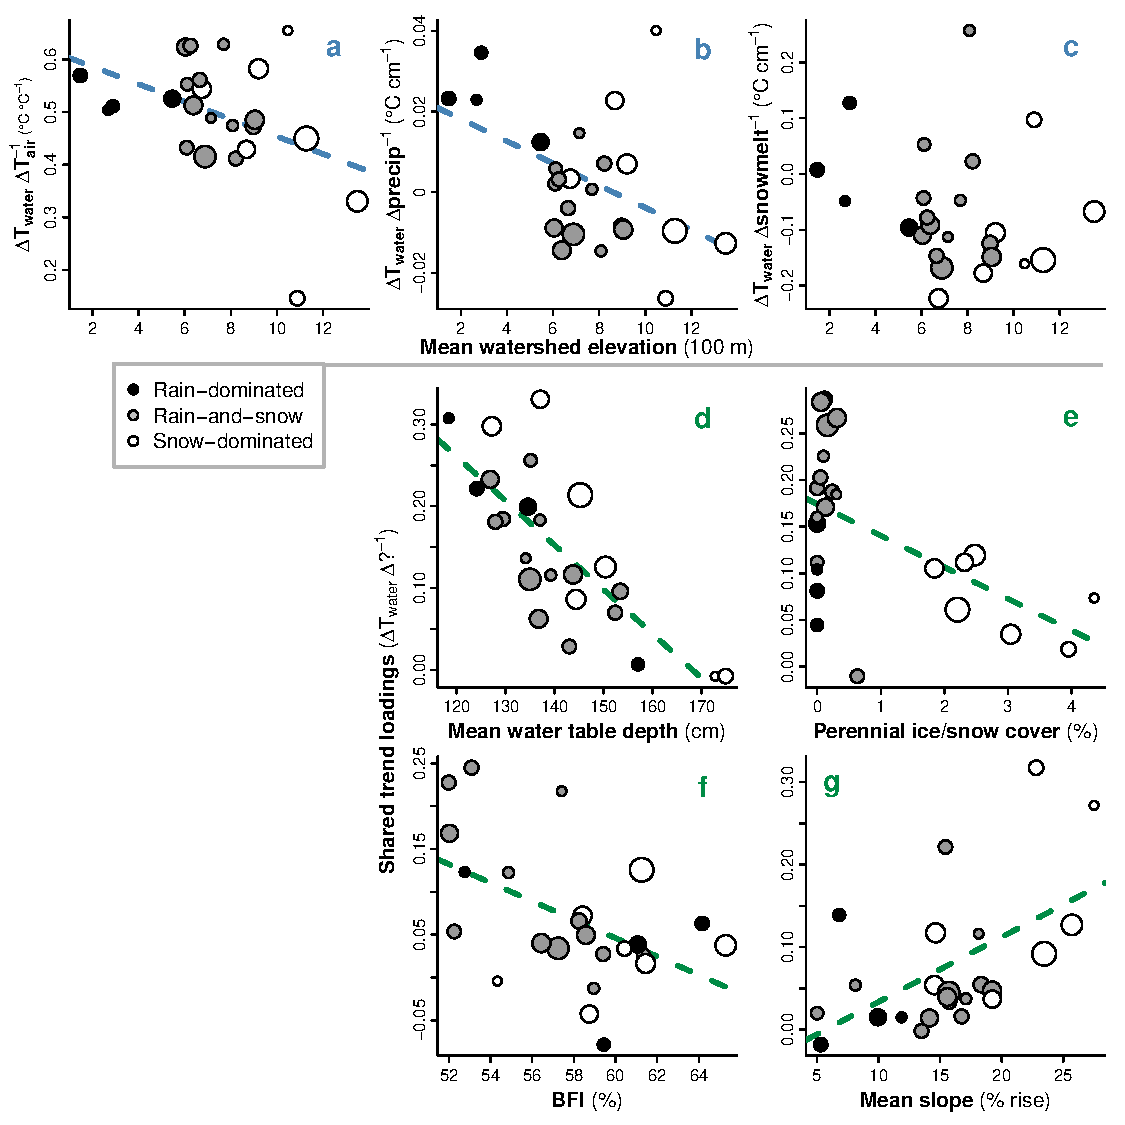
\includegraphics[width=\textwidth]{figures/16_temp_all_reg.pdf}};
    \draw (-4.1, -2.1) node[text width=9.5em] {\normalsize \textbf{Figure 3} Relationships between watershed elevation and climatic effects on T\textsubscript{water} \textbf{(a-c)}, and other watershed predictors and factor loadings on shared trends \textbf{(d-g)}. Points are sized by watershed area. Regression lines indicate slopes significant at $\alpha=0.05$.};
\end{tikzpicture}

In addition to the three climate predictors above, the best T\textsubscript{water} model also included five shared trends. Of these, four correlated significantly with at least one known watershed predictor. Figure 3 depicts the strongest correlated variables with each trend (insets d-e). These are, in arbitrary order of relevance, mean water table depth ($p<0.001, R^2=0.60$; Fig. 3d), \% glaciation ($p<0.01, R^2=0.30$; Fig. 3e), BFI ($p=0.01, R^2=0.25$; Fig. 3f), and mean slope ($p<0.01, R^2=0.29$; Fig. 3g). The fifth shared trend was not correlated with any variables in the watershed predictor dataset.

\begin{center}
\resizebox{\textwidth}{!}{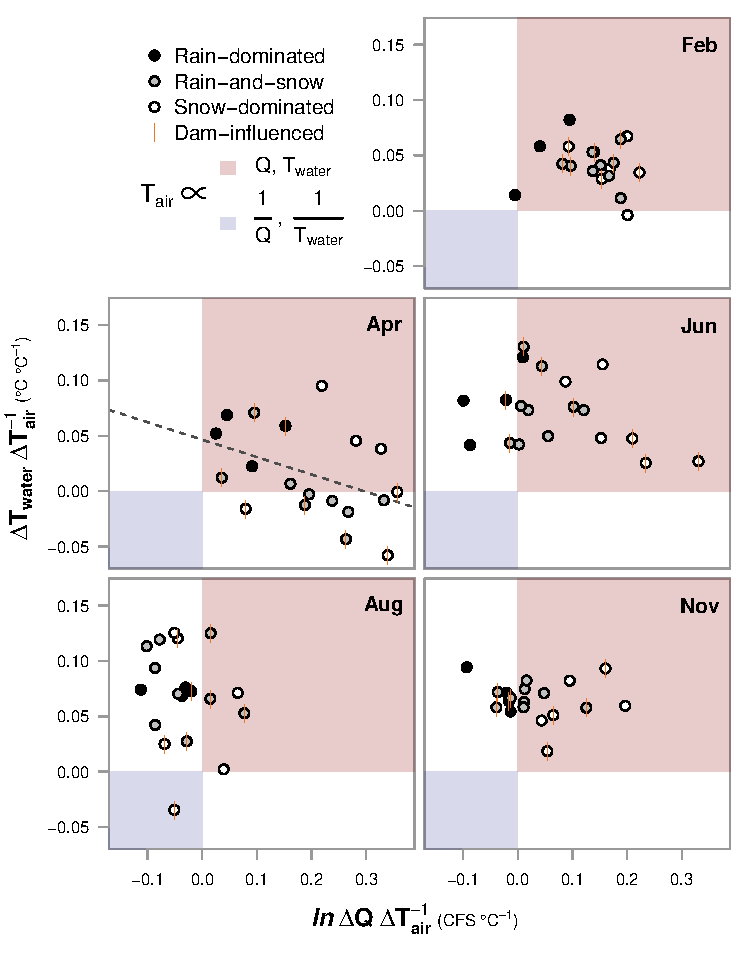
\includegraphics{figures/15_disch_vs_air_focal5.pdf}}
\textbf{Figure 4} Relationship between $T_{air}\rightarrow T_{water}$ and $T_{air}\rightarrow Q$. Both axes are expressed per 1\degree C change in $T_{air}$. The red quadrant designates proportionality between all three variables, the blue inverse proportionality between each response and $T_{air}$. Regression lines indicate slopes significant at $\alpha=0.05$.
\end{center}

To examine possible sub-season interactions between T\textsubscript{air}, T\textsubscript{water} and Q, we performed an additional DFA with Q as the response. In both models, T\textsubscript{air} was allowed to have unique monthly effects. These effects, taken together, can be understood in relation to the four quadrants of the Cartesian coordinate system (increasing clockwise from upper right; Fig. 4).

In mid-winter (exemplified by February), all river classes primarily occupy the first quadrant, signifying $T\textsubscript{air} \propto T\textsubscript{water}$ and $T\textsubscript{air} \propto Q$, where $\propto$ denotes proportionality. RD shows the weakest Q response. By spring, many RS and SD sites develop an inverse relationship between T\textsubscript{air} and T\textsubscript{water}, denoted $T\textsubscript{air} \propto \frac{1}{T\textsubscript{water}}$, while RD sites change little from their winter state. June and August see a procession of most sites into the near fourth quadrant, with SD trailing. This signifies $T\textsubscript{air} \propto \frac{1}{Q}$, though $T\textsubscript{air} \propto T\textsubscript{water}$ remains. One stark exception is again the Elwha river, which occupies quadrant three. By fall, RS and SD have begun progress back toward their winter states, led by SD. RD, meanwhile, remain essentially unmoved from summer.

\section*{Discussion}

The effects of climate on T\textsubscript{water}, determined by dynamic factor analysis, suggest that nearly all rivers included in our dataset were influenced strongly by air temperature, precipitation, and/or snowmelt across 38 years of monthly data (Fig. 3). At most monitoring sites, T\textsubscript{water} closely tracked changes in T\textsubscript{air}, on average responding to increases and decreases with proportional movements of up to 66\% magnitude. However, some rivers only weakly track T\textsubscript{air}, and several patterns in the intensity of this coupling correlate strongly with watershed features relating to ice, groundwater, and slope. Glaciation and yearly snow burden are prominent among these, and for reasons of ecological and hydrological implication, the primary focus of the following discussion.

Without any analysis, a "buffering" effect (hereinafter contrasted with "coupling") of ice on river temperature can be seen in the yearly patterns of \textsubscript{water} relative to T\textsubscript{air} (Fig. 2). The aggregate hydrograph peaks due to snowmelt from April to June, at the same time that the trajectories of RS and SD (snow-influenced rivers) start to drop off relative to RD. After snowmelt begins to subside, RS and SD recover with a noticeable jump. For rivers that receive glacial runoff (SD), this effect appears to remain, buffering them from summer temperature rise where RS rivers instead take on the character of RD (Fig. 4). In an extreme case, the Elwha River was actually cooler in August during those years in which air temperature was higher, likely due to increased runoff from Carrie and Eel glaciers. The buffering effect of ice on river temperature is therefore two-fold, acting first on all snowmelt-influenced rivers through a cold-water pulse in spring, and then on a subset of those rivers throughout summer and fall, by way of glacial runoff. For RD rivers, which receive little to no input from ice, summer temperature is entirely dictated by that of the surrounding air, and whatever rain falls through it. Though higher-elevation watersheds will always produce colder water, independent of the influence of ice, it can be expected that RS and SD rivers will grow more similar to RD as regional temperatures warm and glaciers decline. That is to say, formerly reliably cold-water streams and associated habitats may see increases in both summer and winter average temperatures, as well as higher variability from year to year. The Elwha in particular may slip from its current state of high resistance to seasonal climatic changes. We tested for changes in mean and variance of $T\textsubscript{air}\rightarrow T\textsubscript{water}$ and $T\textsubscript{air}\rightarrow Q$ coupling between 1978 and 2015, but did not detect any regular patterns (Appendix B).

In addition to the three climate predictors, five shared trends were fit by the most parsimonious DFA model. These represent additional drivers responsible for structuring water temperature across some or all of the 24 sites included in the analysis. Each monitoring sites' factor loading on a particular shared trend indicates the degree to which the trend accounted for variance in T\textsubscript{water} at that site. While the precise identities of these drivers cannot be obtained with certainty, they can be inferred through correlation with predictor variables. In this way, we determined the most likely landscape drivers of T\textsubscript{water} to be perennial ice and snow cover, mean watershed slope, and groundwater influx. In the case of slope, the likely mechanism of influence is increased turbulence and mixing of water and air in steep, headwater streams, which allows convective warming and cooling to occur more rapidly \citealt{brutsaert1975theory}; Fig. 3g). As for groundwater, greater influx (represented by baseflow index, or BFI; fig. 3f) corresponds to greater {\it de}-coupling of climatic effects and river temperature, as groundwater should be insulated relative to surface water. For the same reason, greater depth of groundwater should be associated with better insulation and thus further decoupling (Fig. 3d). The buffering effect of perennial ice and snow on SD rivers has already been discussed, but the uniquely high factor loadings of RS rivers in relation to the associated trend are worth noting (Fig. 3e). This trend may account for variation in RS due to traits shared by RD and SD, or to a "rain-on-snow" effect that may yield additional cold water in early spring. The fifth trend did not correlate strongly with any of the landscape predictors in our dataset. It may therefore represent additional, unknown drivers like marine or microclimatic effects, or it may simply account for random noise.

The relationship between climate and river temperature is further influenced by the interaction of discharge, and the fates of rivers in the Puget Sound watershed can be best understood by examining these factors in combination (Fig. 4). Whether rain-, both-, or snow-dominated, all rivers took on RD characteristics in winter, when the effects of ice lay latent. As a result, warmer Februaries on average yielded warmer rivers and higher flow (less precipitation bound in ice). The critical differences between river classes played out in spring and summer, and it's during these months that future purturbations due to changing climate may be felt most acutely. For example, warmer Aprils on average produced colder water at 9 out of 15 RS and SD sites. Though we determined discharge, groundwater, and slope to be likely components of this relationship, only melting ice could be credited with actually reversing it. Projected reductions in snowpack for the Pacific Northwest can therefore be expected to fundamentally alter the responses of currently snow-influenced rivers to yearly variation in spring temperature. In the longer term, changes can be expected for rivers that now receive the temperature-buffering effect of glacial runoff. Glaciers continue to decline across North America, with glacial ice across Western Canada projected to decline by 70\% from 2005 to 2100 \citep{clarke2015projected}.

\section*{Conclusion}

Temperature regimes across the rivers of the Puget Sound watershed are structured by a combination of climatic drivers at the regional scale, and geophysical drivers at watershed scales. In the absence of snow and ice, river temperature is closely coupled to that of the surrounding air, while contributions of snowmelt and glacial runoff can dampen or even reverse this coupling in spring and summer. In some cases, icemelt-influenced rivers exhibit stronger positive responses to climate patterns than their rain-driven counterparts. Our results suggest elevational variations in groundwater influx, total discharge, and watershed slope account for these patterns. However, while these factors may influence the degree of coupling between climatic drivers and water temperature, only snow and ice can reverse it. Since 1978, such reversals have been widespread, particularly during spring melt. Though we did not detect changes in this effect across historical observations, future reductions in snowpack and glacial mass are projected. Consequently, many rivers that now undergo the mildest seasonal temperature changes may be impacted most strongly.
\clearpage

\bibliography{manuscript}
\bibliographystyle{apalike}
\clearpage

\section*{Appendix A}

\subsection*{Temperature DFA output and diagnostics}
Model selection included four climate covariates (air temperature, precipitation, snowmelt, and hydrological drought), between 1 and 15 shared trends, four within-and-among-site error structures (see methods), and two models of unknown seasonal variation (fixed monthly factors and Fourier series). The most parsimonious model of river temperature was selected using the Akaike Information Criterion (AIC), and included air temperature, precipitation, and snowmelt as covariates. This model also included five shared trends and an independent and unequally distributed error structure among streams (i.e. diagonal and unequal variance-covariance matrix).

\begin{center}
\resizebox{\textwidth}{!}{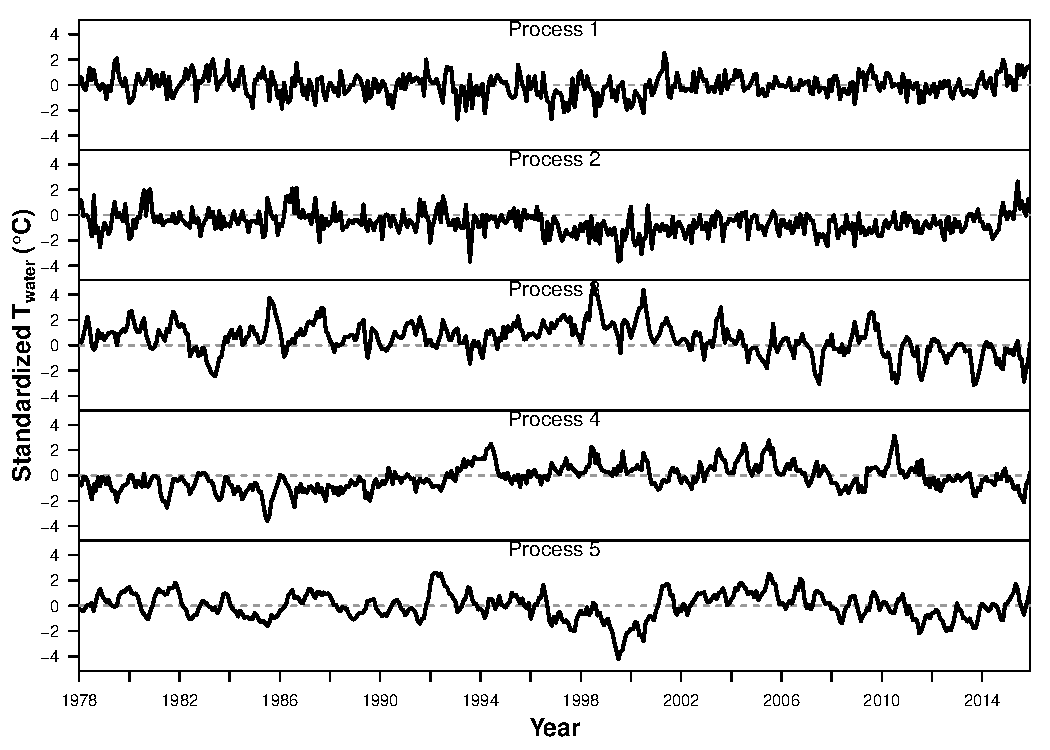
\includegraphics{figures/diagnostic_plots/01_trends.pdf}}
\textbf{Figure A1} Shared trends.
\end{center}

\begin{center}
\resizebox{\textwidth}{!}{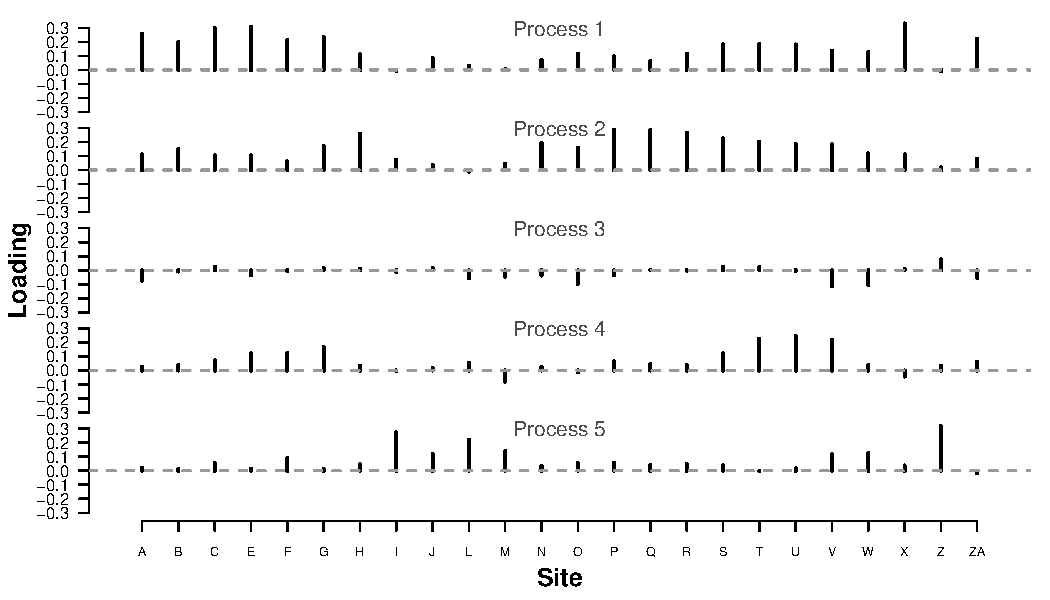
\includegraphics{figures/diagnostic_plots/02_loadings.pdf}}
\textbf{Figure A2} Factor loadings on shared trends.
\end{center}

\begin{center}
\resizebox{\textwidth}{!}{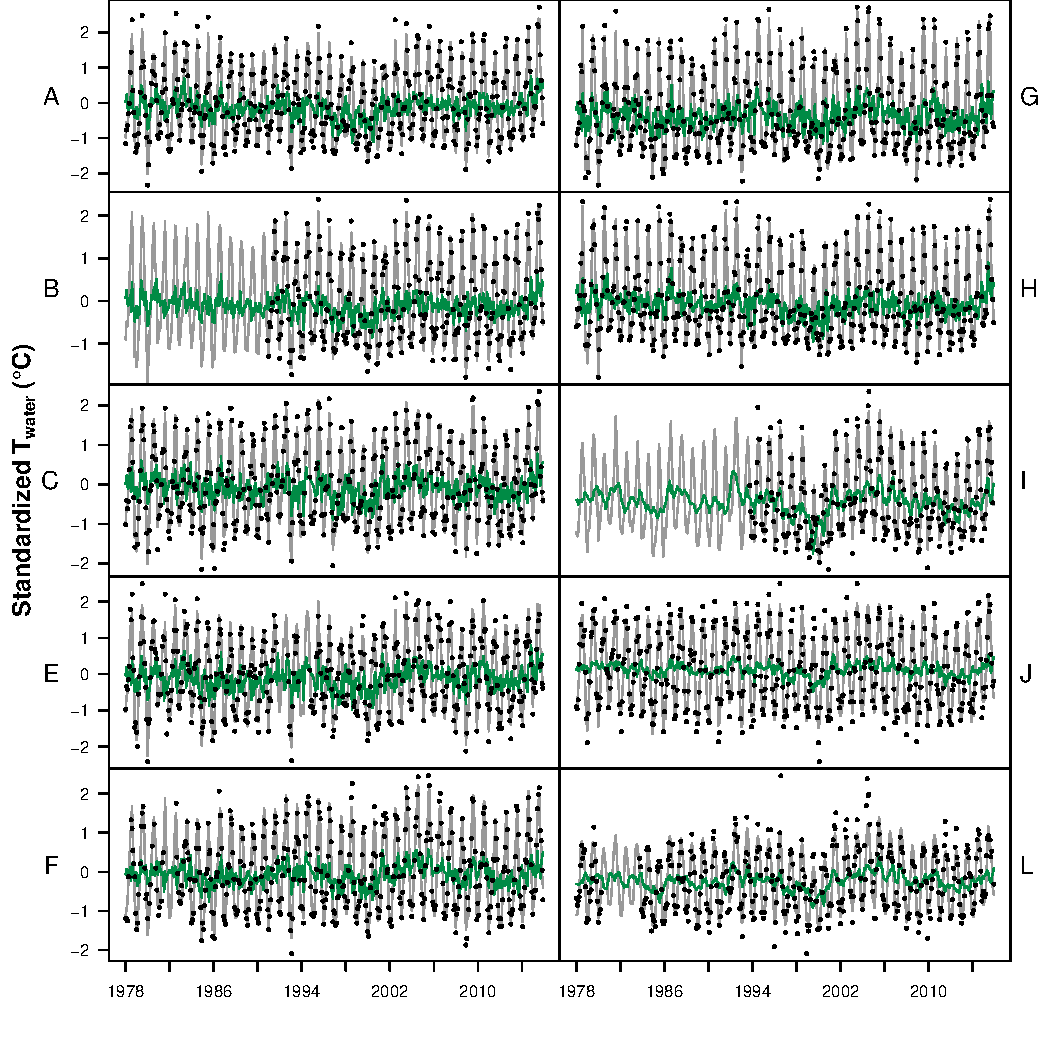
\includegraphics{figures/diagnostic_plots/03_fits.pdf}}
\textbf{Figure A3} Model fits (gray line = overall; black line = trends-only).
\end{center}

\begin{center}
\resizebox{\textwidth}{!}{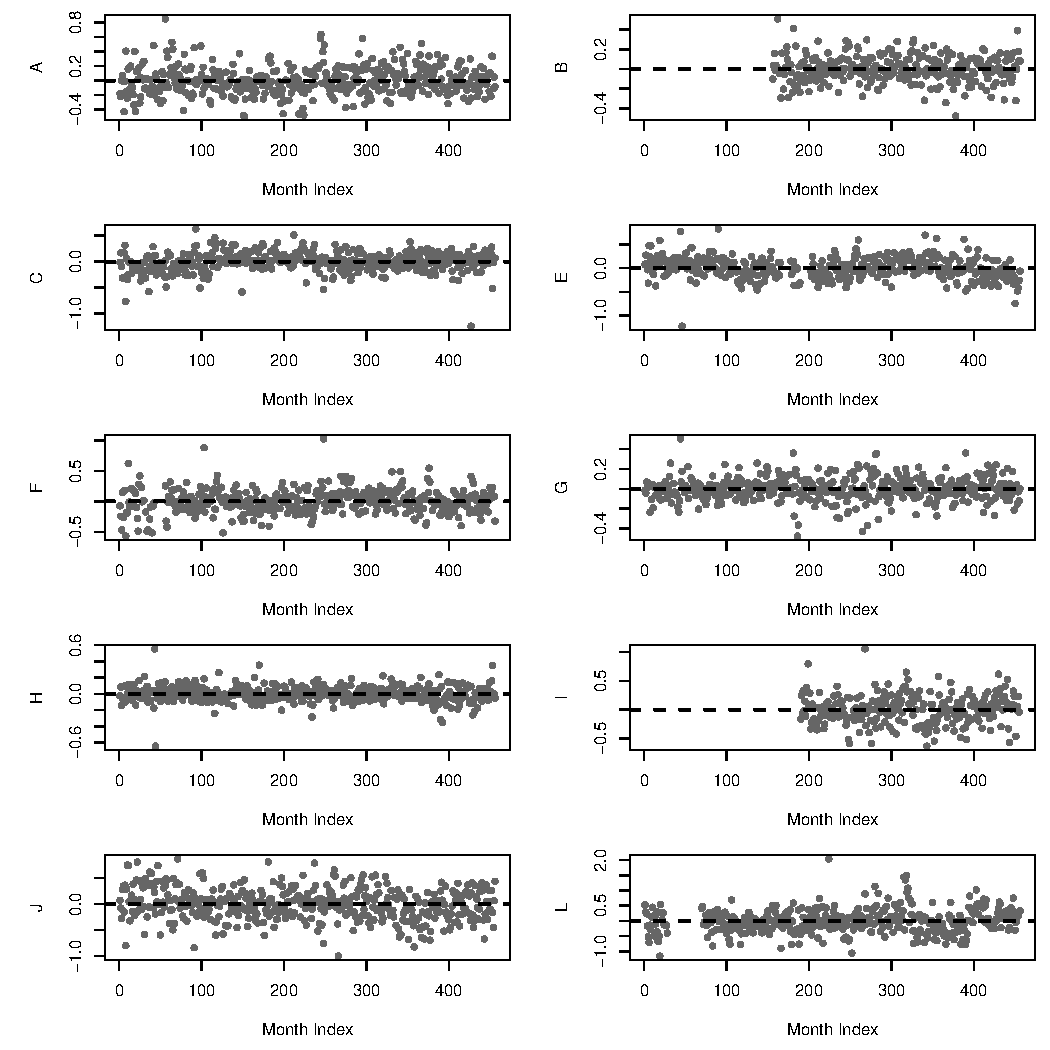
\includegraphics{figures/diagnostic_plots/04_residuals.pdf}}
\textbf{Figure A4} Residuals.
\end{center}

\begin{center}
\resizebox{\textwidth}{!}{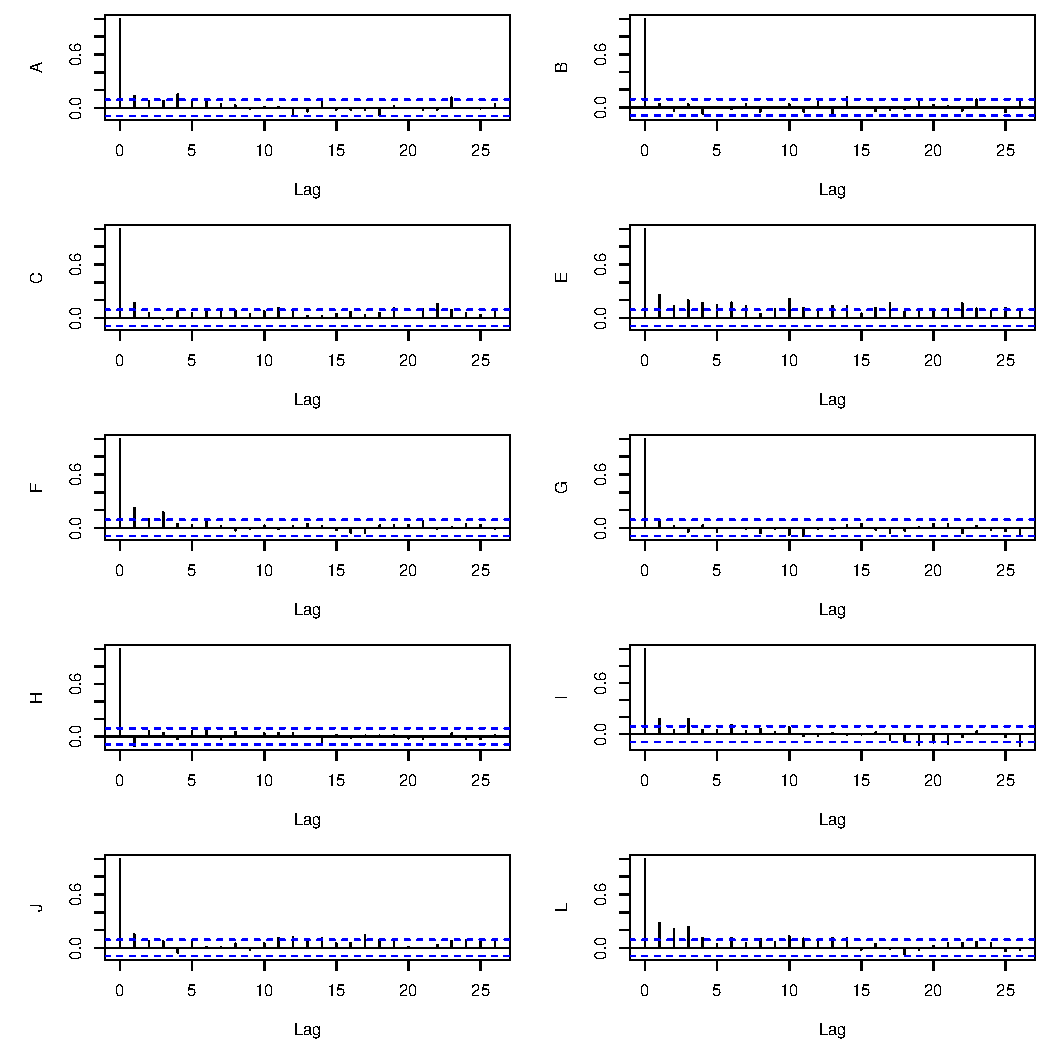
\includegraphics{figures/diagnostic_plots/05_acf.pdf}}
\textbf{Figure A5} Autocovariance function (ACF).
\end{center}

Output from the discharge model looks very similar to this, and is omitted here for the sake of retaining a reasonable page count.
\clearpage

\section*{Appendix B}

\subsection*{Testing for change in coupling over time}

We used an additional DFA model to test for changes in $T_{air}\rightarrow T_{water}$ coupling over time, by dividing the 1978-2015 time series into 5 intervals and comparing central tendency and variance of effect sizes for each interval. Figures B1-B3 show mean effect size for each stream.

To approximate estimates of variability over time, we performed the same analysis within a Bayesian framework, and obtained uncertainty estimates from the credible intervals of the effect size posteriors. This approach yielded no trends in variation over time, and is not visualized here (This will be included in the final version of this paper).

\begin{center}
\resizebox{\textwidth}{!}{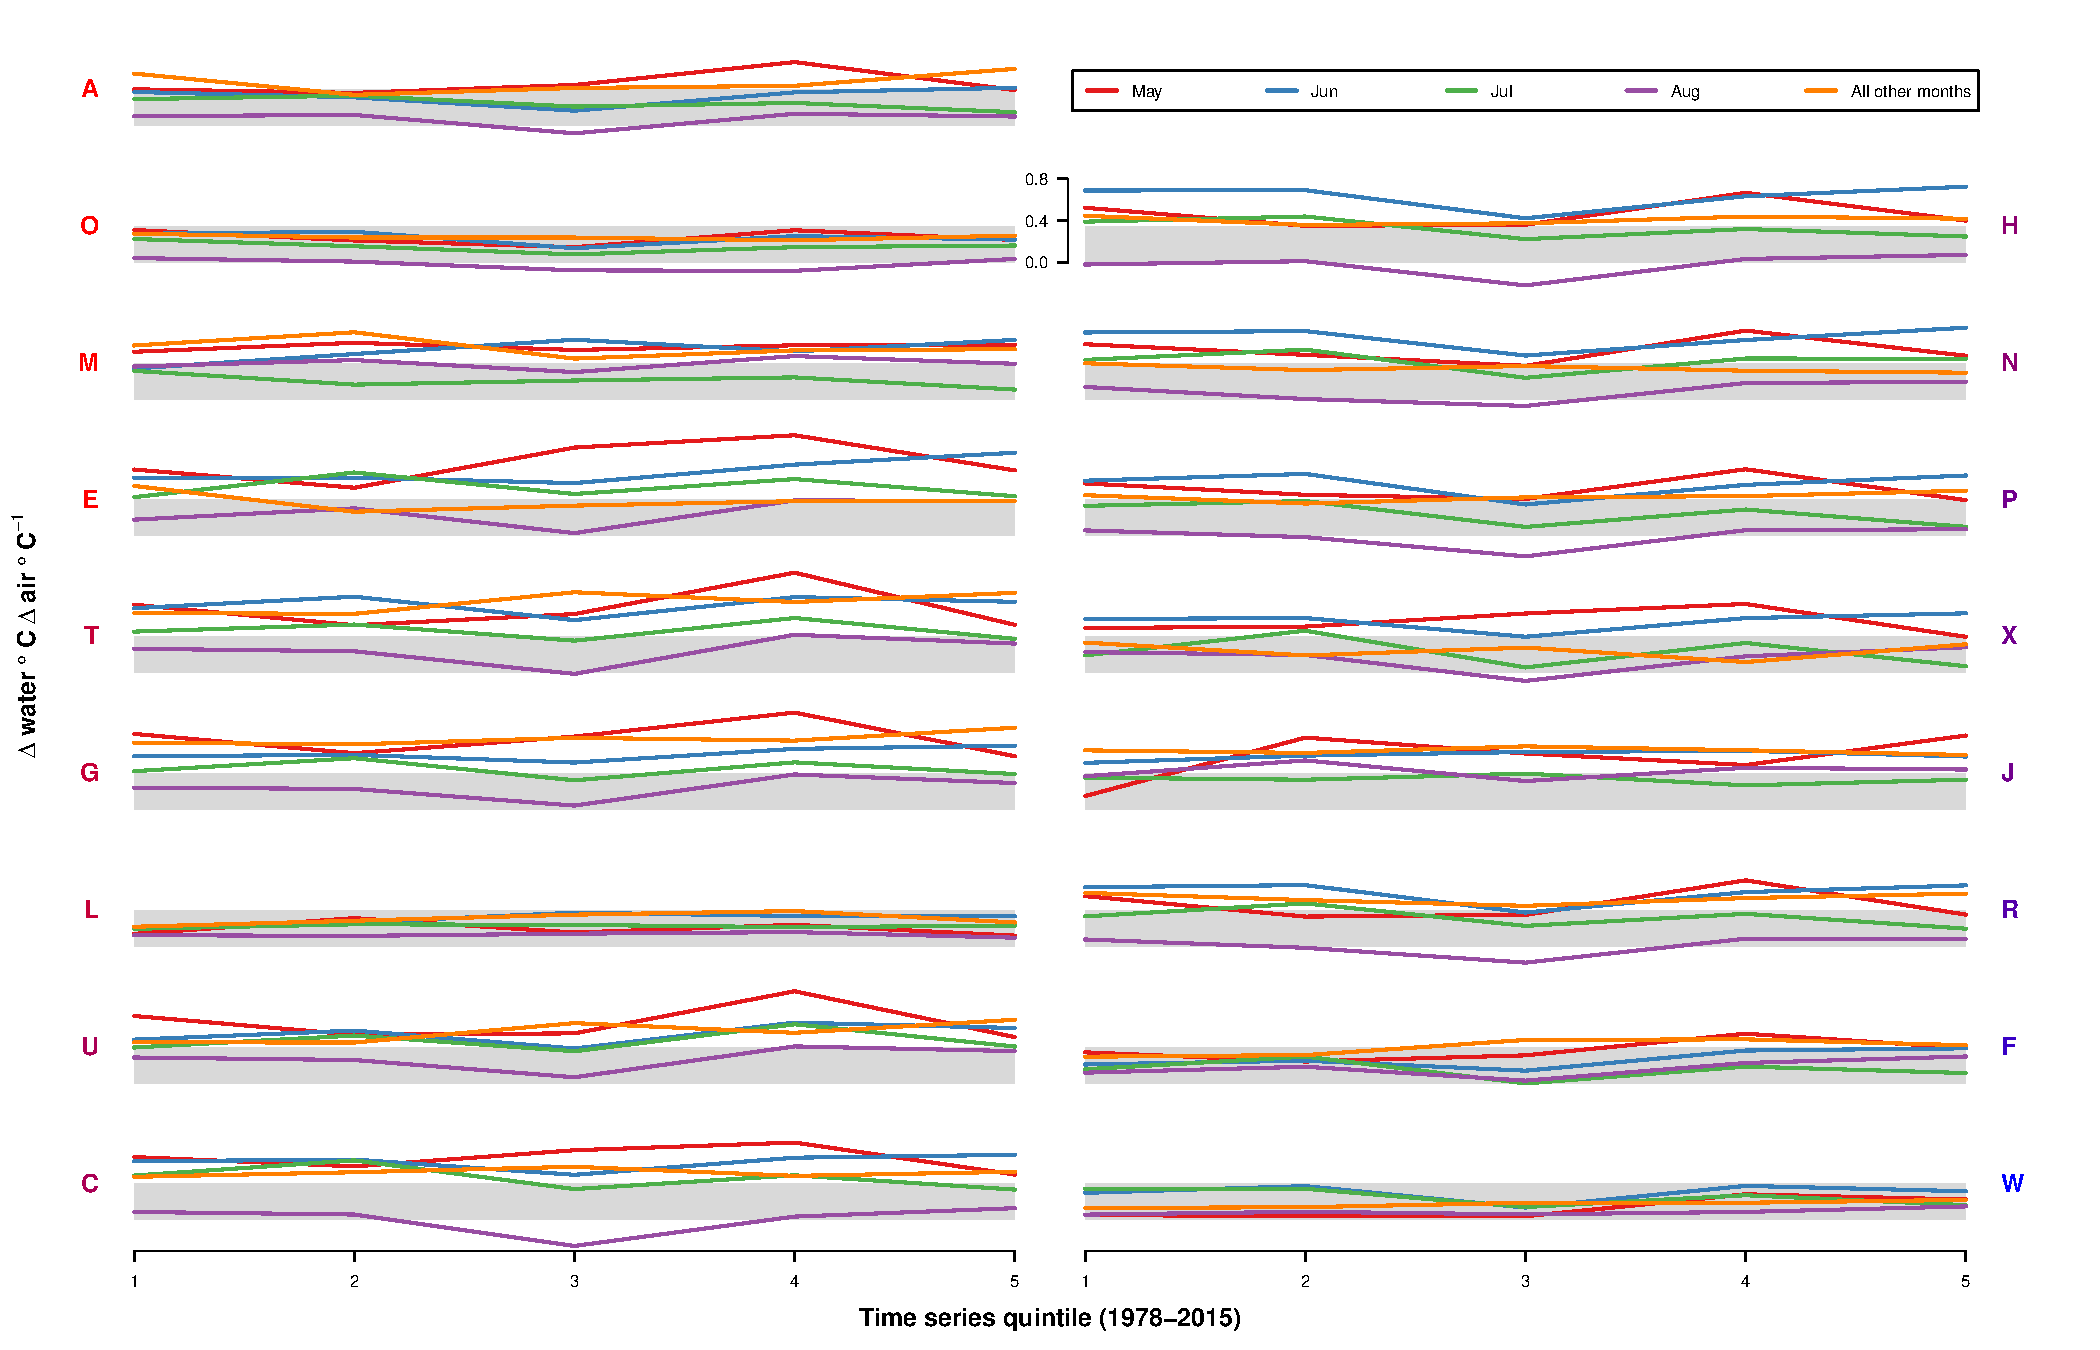
\includegraphics{figures/05a_temp_effSize_byMonth_acrossTime_may-aug.pdf}}
\textbf{Figure B1} Mean $T_{air}\rightarrow T_{water}$ coupling over time. Each plot corresponds to an individual site. Y-label colors represent mean watershed elevation (bluer=higher).
\end{center}

\begin{center}
\resizebox{\textwidth}{!}{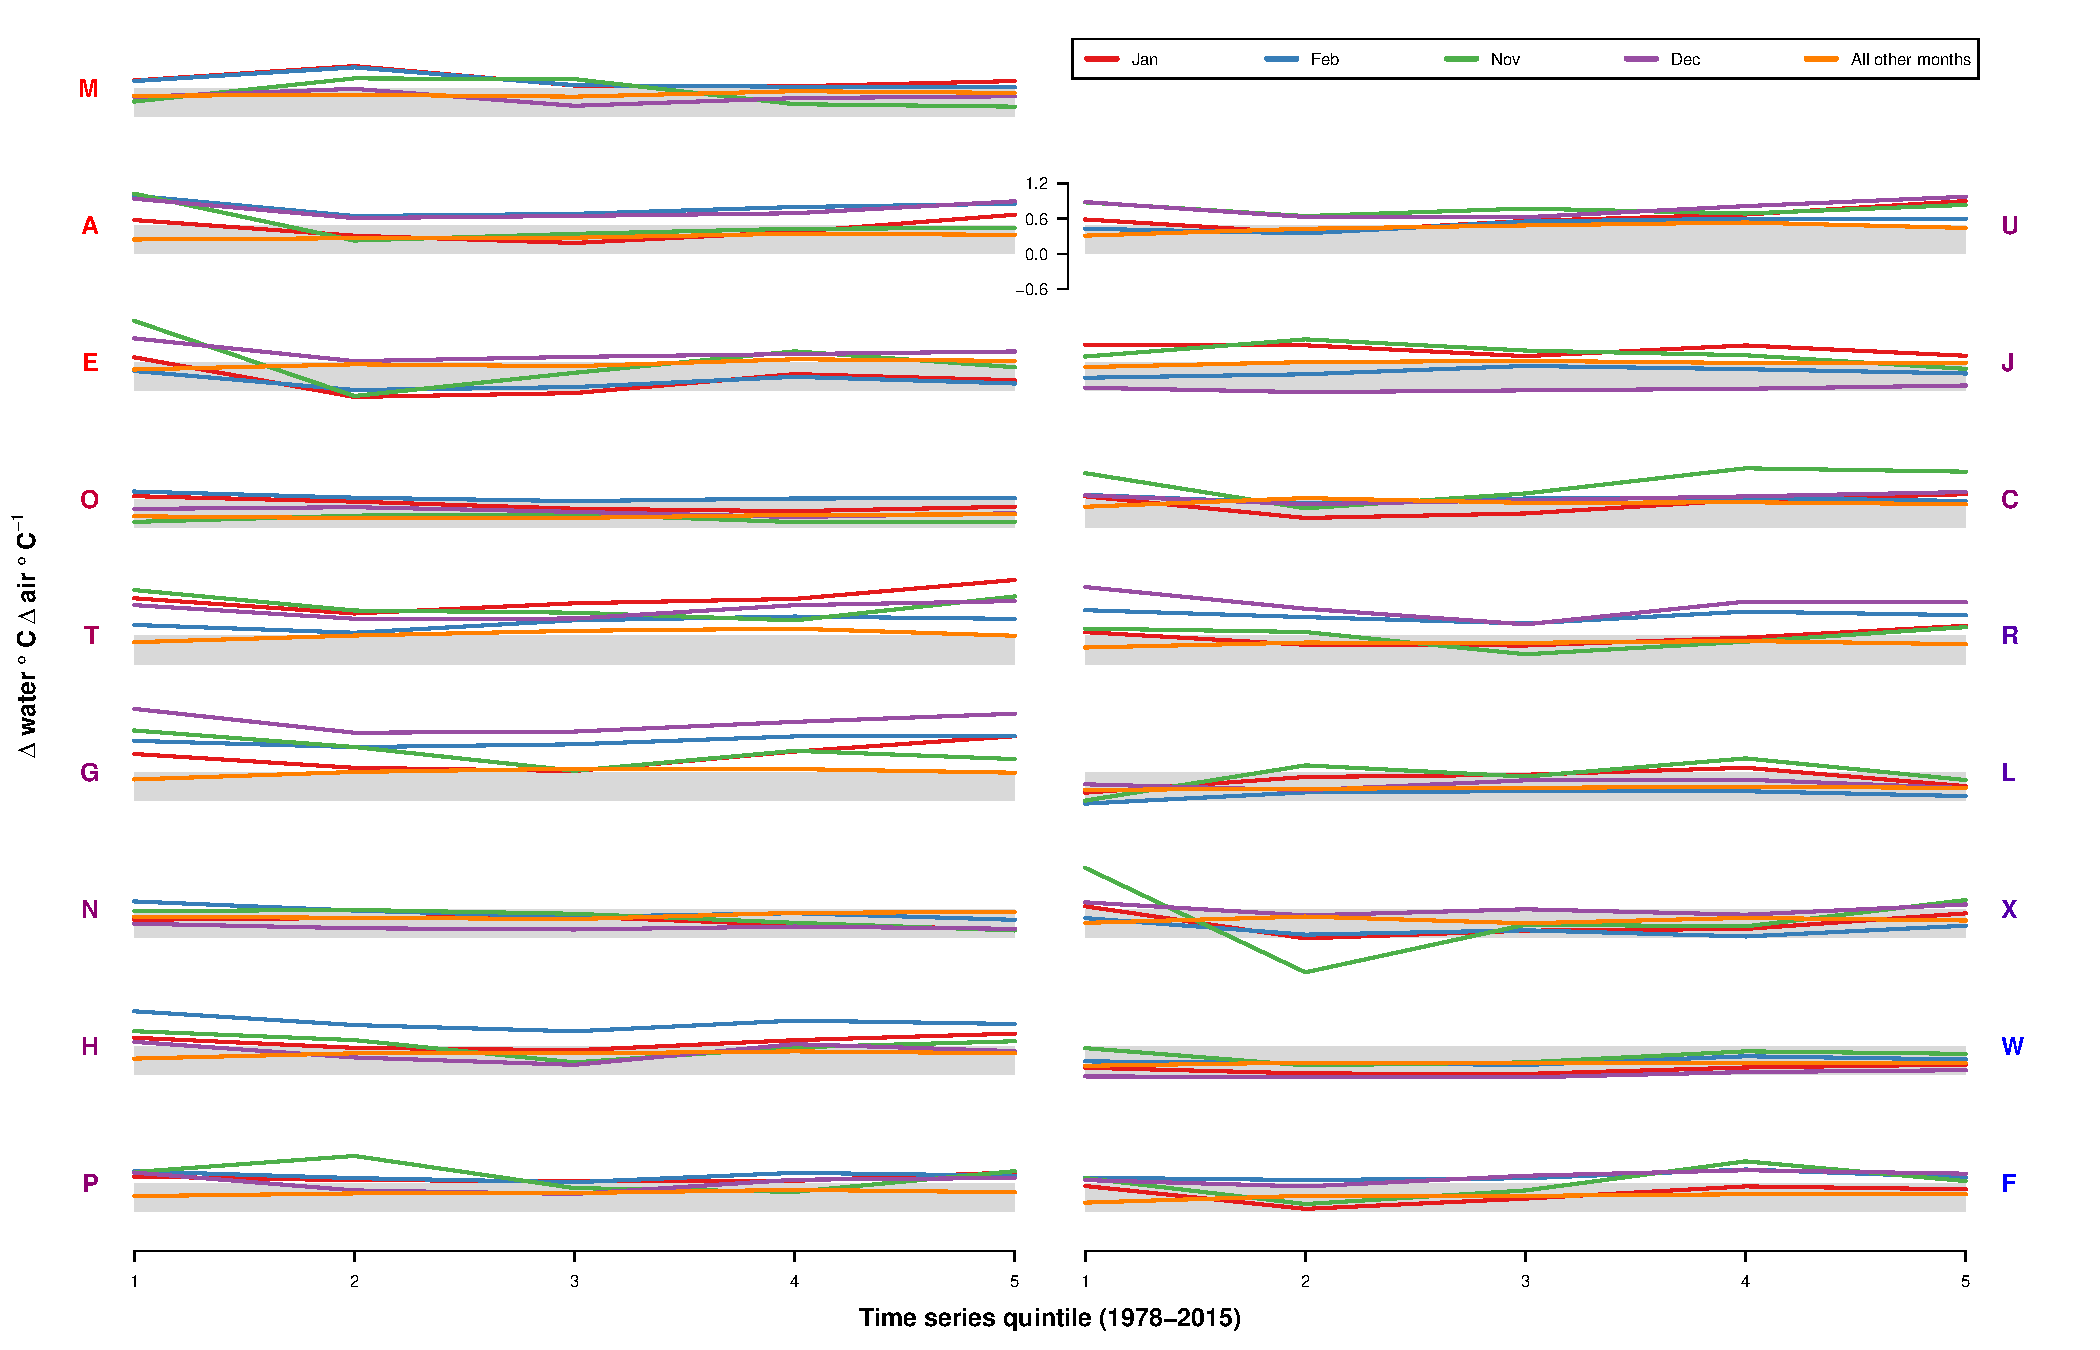
\includegraphics{figures/05b_temp_effSize_byMonth_acrossTime_nov-feb.pdf}}
\textbf{Figure B2} Mean $T_{air}\rightarrow T_{water}$ coupling over time. Each plot corresponds to an individual site. Y-label colors represent mean watershed elevation (bluer=higher).
\end{center}

\begin{center}
\resizebox{\textwidth}{!}{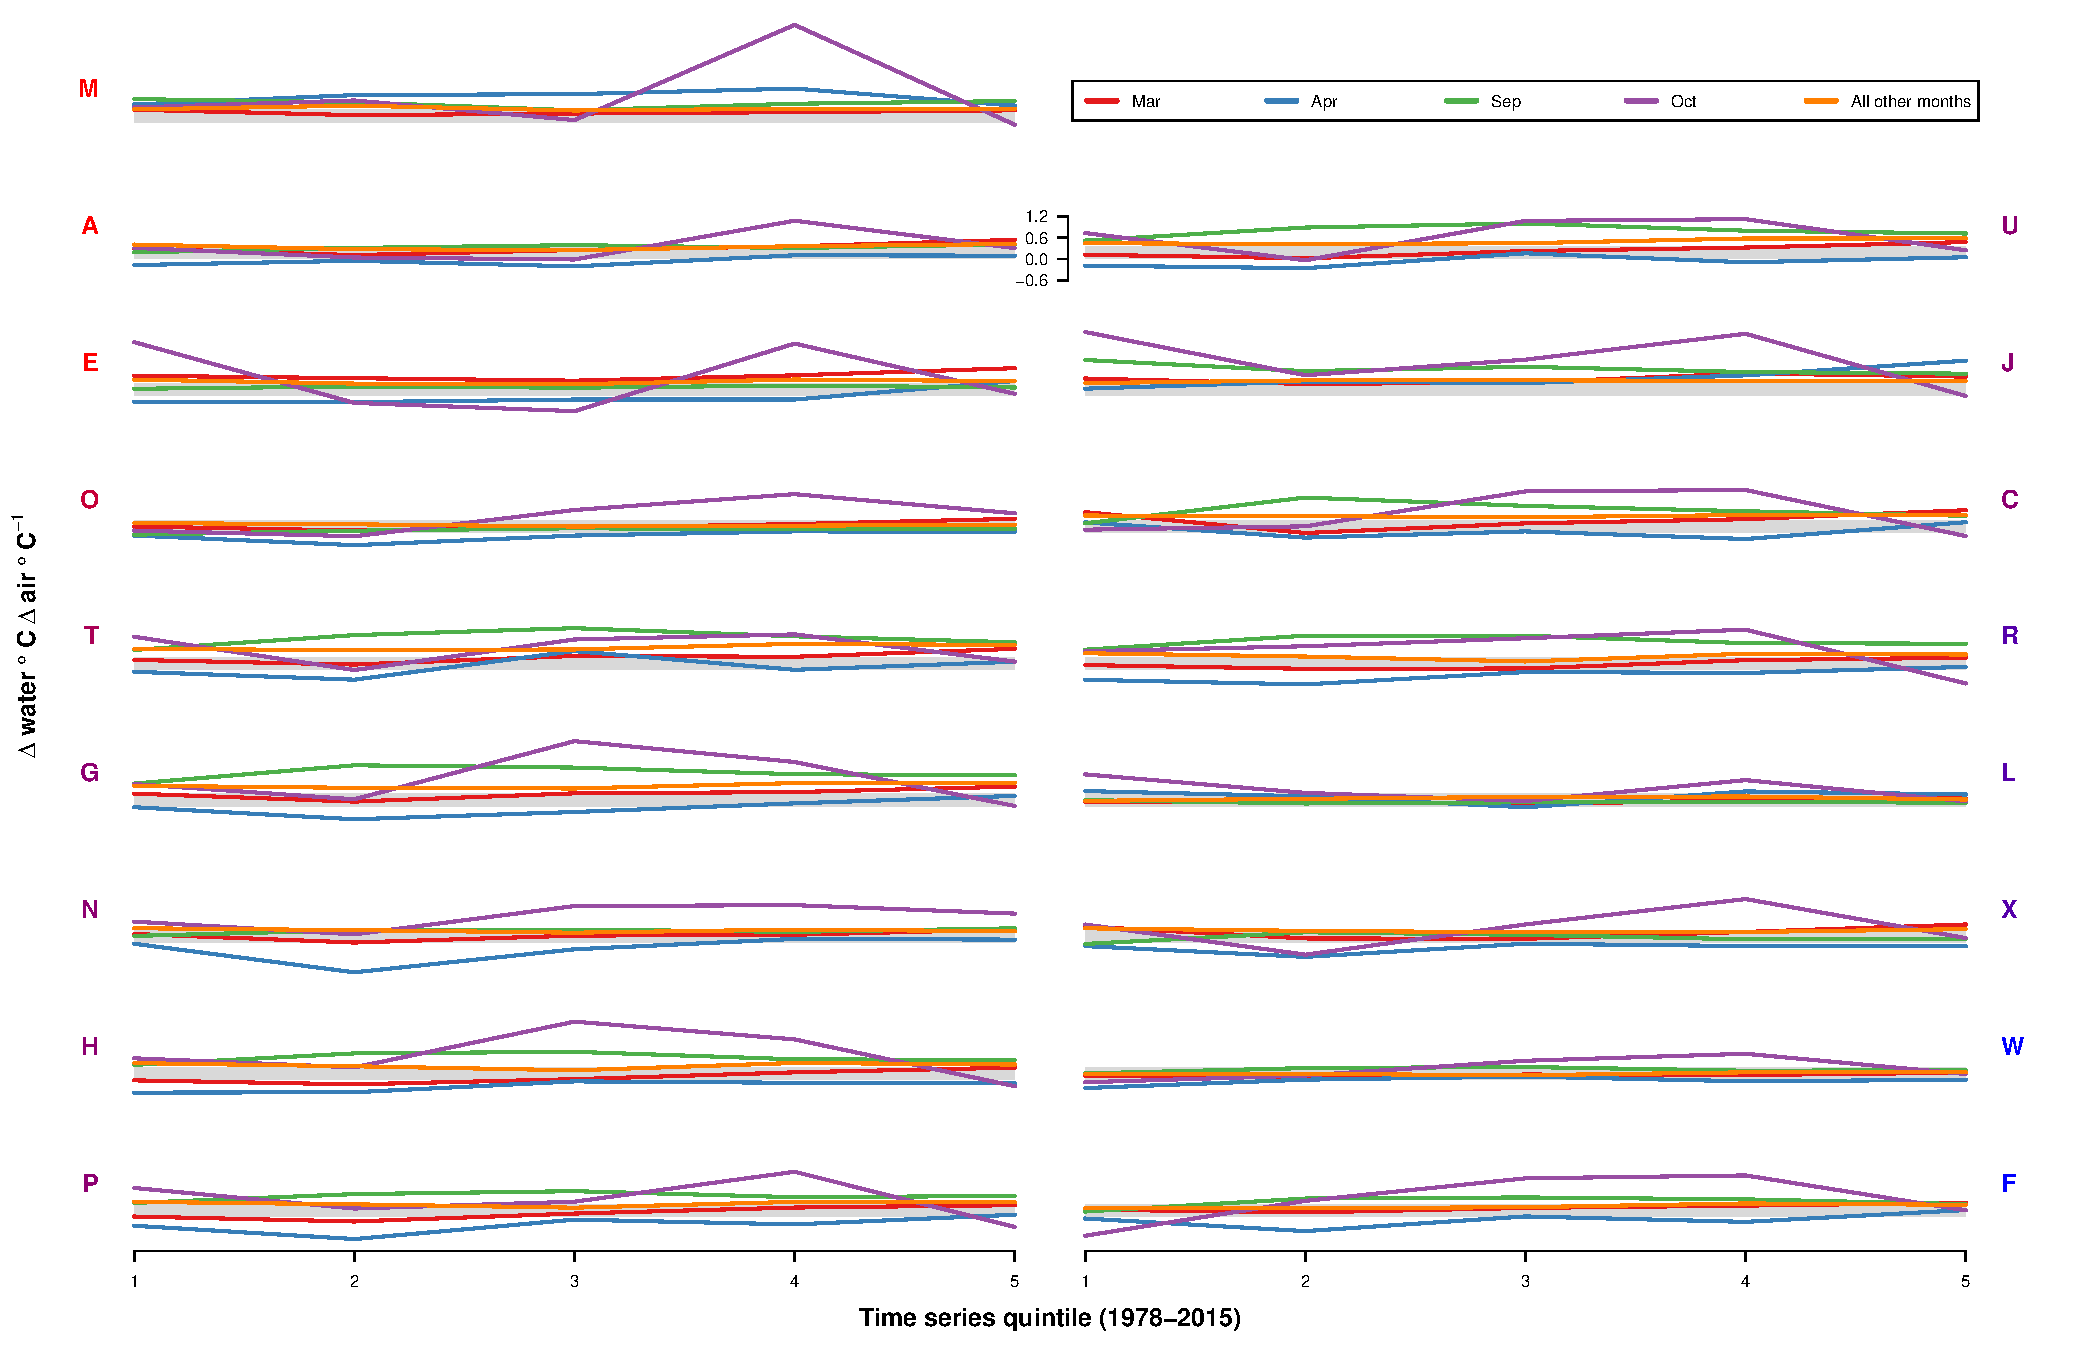
\includegraphics{figures/05c_temp_effSize_byMonth_acrossTime_MASO.pdf}}
\textbf{Figure B3} Mean $T_{air}\rightarrow T_{water}$ coupling over time. Each plot corresponds to an individual site. Y-label colors represent mean watershed elevation (bluer=higher).
\end{center}

\end{document}
